不必要的對象複製可能是C++的低效之處。主要原因是這樣做很簡單,但很難關注到。看一下以下代碼:

\begin{lstlisting}[style=styleCXX]
std::vector<int> v = make_v(… some args …);
do_work(v);
\end{lstlisting}

這個程序中,\texttt{v}被複制了多少次?答案取決於\texttt{make\_v()}和\texttt{do\_work()}函數的實現以及編譯器的優化。這個例子涵蓋了要討論的一些語言細節。

\subsubsubsection{9.3.1\hspace{0.2cm}複製和參數傳遞}

我們將從第二個函數\texttt{do\_work()}開始。若函數以引用(\texttt{const}或非\texttt{const}形式)傳遞實參,則不進行復制。

\begin{lstlisting}[style=styleCXX]
void do_work(std::vector<int>& vr) {
	… vr is a reference to v …
}
\end{lstlisting}

若函數使用按值傳遞,則必須進行復制:

\begin{lstlisting}[style=styleCXX]
void do_work(std::vector<int> vc) {
	… vc is a copy of v …
}
\end{lstlisting}

如果\texttt{vector}對象很大,則複製\texttt{vector}對象的操作代價很高。必須複製\texttt{vector}對象中的所有數據,這是一個代價很高的函數調用。如果不需要\texttt{vector}的副本,那這裡的複製就非常的低效。例如,如果只需要計算\texttt{vector}中所有元素的和(或其他計算),則不需要副本。乍一看,調用本身並沒有告訴我們是否複製,但它應該是這樣的。複製的決定屬於函數的實現者,只有在考慮了需求和算法的選擇後才能做出。對於前面提到的累加所有元素和的問題,正確的決定顯然是通過(\texttt{const})引用傳遞\texttt{vector}對象,如下所示:

\begin{lstlisting}[style=styleCXX]
void do_work(const std::vector<int>& v) {
	int sum = 0;
	for (int x: v) sum += x;
	… use sum … 
}
\end{lstlisting}

使用值傳遞明顯是低效的,並可能會認為是一個Bug,但是這種情況發生的頻率比還挺高。特別是在模板代碼中,作者只考慮了小型、輕量級的數據類型,但代碼最終得到了比預期更廣泛的使用。

另一方面,如果需要創建實參的副本,作為滿足函數要求的一部分,使用參數傳遞是一種很好的方法:

\begin{lstlisting}[style=styleCXX]
	void do_work(std::vector<int> vc) {
		… vc is a copy of v …
	}
\end{lstlisting}

進一步處理數據之前,需要對數據應用一個所謂的固定環。假設多次讀取固定位的值,每次訪問都調用\texttt{std::min()}可能比創建結果的緩存副本的效率要低。也可以顯式的製作一個副本,這可能會更有效,但這種優化不應該只是猜測,需要通過一個基準測試才能明確回答。

C++11引入了移動語義來解決部分不必要的複製。本例中,如果函數實參是右值,可以以任何方式使用,包括修改它(調用者在調用完成後無法訪問該對象)。利用移動語義的常用方法是使用右值引用版本重載函數:

\begin{lstlisting}[style=styleCXX]
void do_work(std::vector<int>&& v) {
	… can alter v data … 
}
\end{lstlisting}

但是,如果對象本身支持移動,簡單的值傳遞版本就有了亮點。參考以下代碼:

\begin{lstlisting}[style=styleCXX]
void do_work(std::vector<int> v) {
	… use v destructively … 
}
std::vector<int> v1(…);
do_work(v1);                 // Local copy is made
do_work(std::vector<int>(…));    // rvalue
\end{lstlisting}

\texttt{do\_work()}的第一次調用使用了左值參數,因此在函數內部進行了局部複製(參數通過值傳遞!)。第二個調用使用右值或未命名的臨時函數,由於\texttt{vector}有一個移動構造函數,函數的實參移動(而不是複製!)到形參中,移動\texttt{vector的}速度非常快。現在,在沒有重載的情況下,通過函數實現,可以有效地處理右值和左值參數,現在已經看到了兩個極端的例子。第一種情況下,不需要副本,顯式的構造一份是低效的。第二種情況下,複製是一種合理的實現。正如即將看到的,並不是每一種情況都屬於這些極端情況。

\subsubsubsection{9.3.2\hspace{0.2cm}使用複製進行實現}

還有一種中間情況,即選擇的實現需要參數的副本,但實現本身並不是最優的。考慮下面的函數,需要按順序輸出:

\hspace*{\fill} \\ %插入空行
\noindent
\textbf{01\_vector\_sort.C}
\begin{lstlisting}[style=styleCXX]
void print_sorted(std::vector<int> v) {
	std::sort(v.begin(), v.end());
	for (int x: v) std::cout << x << “\n”;
}
\end{lstlisting}

對於整數\texttt{vector},這可能是最好的方法,對容器本身進行排序並按順序打印。因為不應該修改原始容器,所以需要一個副本,而且需要利用編譯器來創建一個副本也沒有什麼錯。

但是如果\texttt{vector}的元素不是整數,而是一些大型對象呢?在這種情況下,複製\texttt{vector}就需要佔用大量內存,而對其進行排序需要花費大量時間來複制大型對象。這種情況下,更好的實現可能是在不移動原始對象的情況下,創建指針\texttt{vector}並對其排序:

\hspace*{\fill} \\ %插入空行
\noindent
\textbf{01\_vector\_sort.C}
\begin{lstlisting}[style=styleCXX]
template <typename T>
void print_sorted(const std::vector<T>& v) {
	std::vector<const T*> vp; vp.reserve(v.size());
	for (const T& x: v) vp.push_back(&x);
	std::sort(vp.begin(), vp.end(), 
		[](const T* a, const T* b) { return *a < *b;});
	for (const T* x: vp) std::cout << *x << “\n”;
}
\end{lstlisting}

因為現在已經學會了\textit{永遠不要猜測性能},所以直覺需要通過基準測試來確認。因為對已經排序的\texttt{vector}進行排序不需要任何複製,所以希望在基準測試的每次迭代中都有一個新的、未排序的\texttt{vector},如下所示:

\hspace*{\fill} \\ %插入空行
\noindent
\textbf{01\_vector\_sort.C}
\begin{lstlisting}[style=styleCXX]
void BM_sort(benchmark::State& state) {
	const size_t N = state.range(0);
	std::vector<int> v0(N); for (int& x: v0) x = rand();
	std::vector<int> v(N);
	for (auto _ : state) {
		v = v0;
		print_sorted(v);
	}
	state.SetItemsProcessed(state.iterations()*N);
}
\end{lstlisting}

當然,應該禁用打印,因為對I/O基準測試不感興趣。另一方面,應該在不進行排序的情況下對複製\texttt{vector}進行基準測試,這樣就可以知道所測量的時間的哪一部分花在了準備測試上。

基準測試確認,對於整數,複製整個\texttt{vector}對象並對其進行排序會更快:

%\hspace*{\fill} \\ %插入空行
\begin{center}
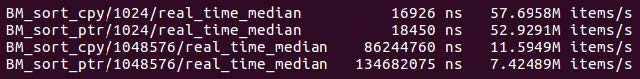
\includegraphics[width=0.9\textwidth]{content/3/chapter9/images/1.jpg}\\
圖9.1 - 對整數\texttt{vector}排序的基準測試:複製方式和指針方式(間接)的對比
\end{center}

請注意,如果數組很小,而且所有數據都適合底層緩存,那麼無論哪種方式,處理速度都非常快,而且速度差異很小。如果對象比較大,複製的代價也比較高,那麼間接性方式就會比較高效:

%\hspace*{\fill} \\ %插入空行
\begin{center}
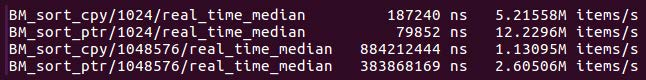
\includegraphics[width=0.9\textwidth]{content/3/chapter9/images/2.jpg}\\
圖9.2 - 大型對象的\texttt{vector}排序基準測試:複製方式和指針(間接)方式
\end{center}

還有一種特殊情況,即實現時需要複製對象。

\subsubsubsection{9.3.3\hspace{0.2cm}複製存儲數據}

C++中會遇到另一種數據複製的特殊情況。這種情況最常發生在類構造函數中,在類構造函數中,對象必須存儲數據的副本,因此必須創建一個生命週期超過構造函數調用生命週期的副本。看一下這個例子:

\begin{lstlisting}[style=styleCXX]
class C {
	std::vector<int> v_;
	C(std::vector<int> ??? v) { … v_ is a copy of v … }
};
\end{lstlisting}

這裡的目的是複製一份,低效率的做法是複製多箇中間副本或一個不必要的副本。實現的標準方法是通過\texttt{const}引用獲取對象,並在類內部複製:

\begin{lstlisting}[style=styleCXX]
class C {
	std::vector<int> v_;
	C(const std::vector<int>& v) : v_(v) { … }
};
\end{lstlisting}

如果構造函數的實參是左值,這是最高效的。但是,如果實參是右值(臨時值),可以將它移到類中,從而不進行復制。這需要重載構造函數:

\begin{lstlisting}[style=styleCXX]
class C {
	std::vector<int> v_;
	C(std::vector<int>&& v) : v_(std::move(v)) { … }
};
\end{lstlisting}

缺點是需要編寫兩個構造函數,但如果構造函數有幾個參數,並且每個參數都需要複製或移動,情況就麻煩了。按照這種模式,將需要6個構造函數重載來處理3個參數。

另一種方法是按值傳遞所有參數,並移動參數。看下代碼:

\begin{lstlisting}[style=styleCXX]
class C {
	std::vector<int> v_;
	C(std::vector<int> v) : v_(std::move(v)) 
	{ … do not use v here!!! … }
};
\end{lstlisting}

形參\texttt{v}現在是一個處於已移動狀態的對象,不應該在構造函數體中再使用。如果實參是左值,則創建一個副本來構造形參\texttt{v},然後移動到類中。如果實參是右值,則將其移動到形參\texttt{v}中,然後再次移動到類中。如果移動成本較低,這種模式就很高效。然而,如果對象的移動代價很高,或者根本沒有移動構造函數(只能複製),最終則會進行兩次複製,而不是一次。 

我們關注的是將數據放入函數和對象的問題。但是當需要返回結果時,複製也可能發生。這裡的考慮因素完全不同,需要分別研究。

\subsubsubsection{9.3.4\hspace{0.2cm}複製返回值}

本節開頭的示例包含了這兩種類型的複製。特別是這一行:

\begin{lstlisting}[style=styleCXX]
std::vector<int> v = make_v(… some args …);
\end{lstlisting}

生成的\texttt{v}是由\texttt{make\_v}函數返回的:

\hspace*{\fill} \\ %插入空行
\noindent
\textbf{02\_rvo.C}
\begin{lstlisting}[style=styleCXX]
std::vector<int> make_v(… some args …) {
	std::vector<int> vtmp;
	… add data to vtmp …
	return vtmp;
}
\end{lstlisting}

理論上,這裡可以進行不止一次的複製:局部變量\texttt{vtmp}複製到\texttt{make\_v}函數的(未命名)返回值中,又複製到最終結果\texttt{v}中。首先,\texttt{make\_v}的臨時返回值會移動,而不是複製到\texttt{v}中。但即使是這樣,也可能不會發生。如果用自己的類,而不是\texttt{std::vector}來嘗試這段代碼,會看到這裡既沒有使用複製構造函數,也沒有使用移動構造函數:

\hspace*{\fill} \\ %插入空行
\noindent
\textbf{02\_rvo.C}
\begin{lstlisting}[style=styleCXX]
class C {
	int i_ = 0;
	public:
	explicit C(int i) : i_(i) { 
		std::cout << “C() @” << this << std::endl;
	}
	C(const C& c) : i_(c.i_) {
		std::cout << “C(const C&) @” << this << std::endl;
	}
	C(C&& c) : i_(c.i_) {
		std::cout << “C(C&&) @” << this << std::endl;
	}
	~C() { cout << “~C() @” << this << endl; }
	friend std::ostream& operator<<( std::ostream& out,
	const C& c) {
		out << c.i_; return out;
	}
};  
C makeC(int i) { C ctmp(i); return ctmp; }
int main() {
	C c = makeC(42);
	cout << c << endl;
}
\end{lstlisting}

這個程序輸出如下內容(對於大多數編譯器,必須開啟某種級別的優化):

%\hspace*{\fill} \\ %插入空行
\begin{center}
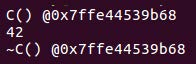
\includegraphics[width=0.4\textwidth]{content/3/chapter9/images/3.jpg}\\
圖9.3 - 程序按值返回一個對象的輸出
\end{center}

只構造和銷燬了一個對象,這是編譯器優化的結果。這裡使用的優化為\textbf{返回值優化(RVO)},編譯器認識到所涉及的三個對象——局部變量\texttt{ctmp}、未命名的臨時返回值和最終結果\texttt{c}——都是相同的類型。此外,編寫的代碼都不可能同時觀察到這兩個變量。因此,在不改變可觀察行為的情況下,編譯器可以為這三個變量使用相同的內存位置。調用函數之前,編譯器需要分配用於構造最終結果\texttt{c}的內存。這個內存地址由編譯器傳遞到函數中,用於在相同的位置構造局部變量\texttt{ctmp}。因此,當函數\texttt{makeC}結束時,根本不需要返回任何東西,結果已經在它應該在的地方了。這就是RVO。

雖然RVO看起來很簡單,但它有幾個微妙之處。 

首先,這是一種優化。這意味著編譯器通常不必這樣做(如果編譯器不這樣做,可能需要一個更好的編譯器),這是一種非常特殊的優化。通常,編譯器可以對程序做任何事情,只要不改變可觀察對象的行為。可觀察行為包括輸入、輸出和訪問易失性存儲器。然而,這種優化導致了一個可觀察的變化,複製構造函數和匹配的析構函數的預期輸出不見了。實際上,這是一個例外:編譯器允許消除複製或移動構造函數和相應的析構函數的調用,即使這些函數有包含可觀察行為的副作用,並且這個例外不侷限於RVO。通常,不能僅僅因為編寫了一些似乎在進行復制的代碼,就指望調用複製和移動構造函數。這就是所謂的\textbf{忽略複製}(或對於移動構造函數來說,就是\textbf{忽略移動})。

其次,(再次)這是一種優化。代碼必須先編譯,然後才能進行優化。如果對象沒有任何複製或移動構造函數,這段代碼將無法編譯,所以將永遠不會進入優化步驟,該步驟將刪除所有對這些構造函數的調用。若在我們的例子中刪除了所有的複製和移動構造函數,就很容易得到失敗的結果:

\begin{lstlisting}[style=styleCXX]
class C {
	…
	C(const C& c) = delete;
	C(C&& c) = delete;
}; 
\end{lstlisting}

編譯現在會失敗,確切的錯誤信息取決於編譯器和C++標準級別。在C++17中,看起來是這樣的:

%\hspace*{\fill} \\ %插入空行
\begin{center}
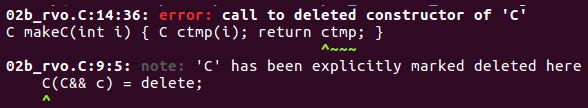
\includegraphics[width=0.9\textwidth]{content/3/chapter9/images/4.jpg}\\
圖9.4 - 使用Clang(支持C++17或C++20)編譯的輸出
\end{center}

特殊情況是,即使刪除了複製和移動操作,程序仍然可以編譯。稍微修改一下\texttt{makeC}函數:

\begin{lstlisting}[style=styleCXX]
C makeC(int i) { return C(i); }
\end{lstlisting}

C++11和C++14沒有什麼變化。然而,在C++17及以上版本中,這段代碼可以很好地編譯。注意,與前一個版本的差別:返回的對象過去是左值,它有一個名稱。現在它是一個右值,一個未命名的臨時值。雖然\textbf{命名RVO(NRVO)}仍然是一種優化,但未命名RVO是強制性的,因為C++17不再認為其是一個忽略複製。該標準規定,一開始就不要求複製或移動。 

最後,可能想知道是否必須使用內聯函數,以便編譯器在編譯函數本身時知道返回值在哪裡。可以進行一個簡單的測試,可以確信事實並非如此:即使函數\texttt{makeC}位於單獨的編譯單元中,RVO仍然會發生。因此,編譯器必須將結果的地址發送到函數的調用點。如果不返回函數的結果,而是將結果的引用作為附加參數傳遞,開發者也可以做類似的事情。當然,必須首先構造該對象,而編譯器生成的優化不需要額外的構造函數調用。 

可能會看到不依賴RVO的建議,但會強制執行返回值的移動:

\begin{lstlisting}[style=styleCXX]
C makeC(int i) { C c(i); return std::move(c); }
\end{lstlisting}

如果RVO沒有發生,程序將承擔複製操作的性能損失,而移動操作顯然是更好的選擇。然而,這種觀點是錯誤的。要理解原因,請仔細查看圖9.4中的錯誤消息:編譯器報錯說移動構造函數刪除了,儘管\texttt{ctmp}是左值,並應該複製。這不是編譯器的錯誤,但反映了標準所要求的行為。在返回值時進行優化是可能的,但編譯器決定是否這麼做取決於上下文,編譯器必須首先找到一個移動構造函數來返回結果。如果沒有找到移動構造函數,則執行第二次查找。這一次,編譯器會尋找複製構造函數。在這兩種情況下,編譯器實際上是在執行重載解析,因為對象可以有許多複製或移動構造函數。因此,沒有理由寫一個顯式的移動,編譯器將自己生成一個。但這有什麼不好的呢?其危害在於,使用顯式移動將禁用RVO。需要一個移動,那麼就獲得一個。雖然移動可能只需要很少的工作,但RVO根本沒有工作量,而且不工作總是比有工作快。

如果刪除了移動構造函數,而沒有刪除複製構造函數,會發生什麼?如果兩個構造函數都刪除了,編譯仍然會失敗。聲明一個已刪除的成員函數,與不聲明任何成員函數是不同的。如果編譯器對移動構造函數執行重載解析,將找到一個移動構造函數(即使這個構造函數被刪除了)。編譯失敗的原因是,因為重載解析選擇一個已刪除的函數作為最佳(或唯一)重載。如果想強制使用複製構造函數(當然是以科研的名義),就不必聲明任何移動構造函數。 

現在,已經看到了隱藏在代碼中的複製對象,從而會有拉低程序性能的危險。能做些什麼來避免無意的複製嗎?我們稍後會給出一些建議,但先讓我們回到已經使用過的一種方法:指針。

\subsubsubsection{9.3.5\hspace{0.2cm}使用指針避免複製}

傳遞對象時避免複製對象的一種方法是傳遞指針。如果不需要管理對象的生命週期,那這是最簡單的方式。如果函數需要訪問一個對象,但不需要刪除它,那麼通過引用或原始指針傳遞對象是最好的方式(在上下文中,引用實際上只是一個不能為空的指針)。 

類似地,可以使用指針從函數返回一個對象,但這需要注意一些問題。首先,對象必須在堆上分配。絕對不能返回指向局部變量的指針或引用。參考以下代碼:

\begin{lstlisting}[style=styleCXX]
C& makeC(int i) { C c(i); return c; } // Never do this!
\end{lstlisting}

其次,調用者負責刪除對象,因此函數的每個調用者都必須知道對象是如何構造的(\texttt{new}操作符不是構造對象的唯一方法,不過是最常見的方法而已)。這裡的最佳解決方案是返回智能指針:

\hspace*{\fill} \\ %插入空行
\noindent
\textbf{03\_factory.C}
\begin{lstlisting}[style=styleCXX]
std::unique_ptr<C> makeC(int i) {
	return std::make_unique<C>(i);
}
\end{lstlisting}

注意,這樣的工廠函數應該返回唯一指針,即使調用者可以使用共享指針來管理對象的生命週期:從唯一指針移動到共享指針很容易,成本也很低。

說到共享指針,它們通常用於傳遞生命期由智能指針管理的對象。除非目的是同時傳遞對象的所有權,否則這又是一個不必要和低效的複製的例子。複製共享指針開銷也不小。若我們有一個由共享指針管理的對象,以及一個需要操作這個對象而不需要佔有它的函數,應該怎麼辦呢?就可以使用原始指針:

\begin{lstlisting}[style=styleCXX]
void do_work1(C* c);
void do_work2(const C* c);
std::shared_ptr<C> p { new C(…) };
do_work1(&*p);
do_work2(&*p);
\end{lstlisting}

函數\texttt{do\_work1()}和\texttt{do\_work2()}的聲明告訴我們開發者的意圖,這兩個函數都操作對象而不刪除它。第一個函數修改對象,第二個則不然。這兩個函數都希望在沒有對象的情況下調用,並將處理這種特殊情況(否則,參數將通過引用傳遞)。 

類似地,只要對象的生命週期是在別處管理,就可以創建原始指針的容器。如果希望容器管理其元素的生命週期,但又不想將對象存儲在容器中,可以則使用具有唯一指針的容器來完成這項工作。 

現在是時候給出一些通用的指導指南了,這些指導指南將幫助我們避免不必要的複製,以及相應的低效率。

\subsubsubsection{9.3.6\hspace{0.2cm}如何避免不必要的複製}

也許為了減少意外的、無意義的複製,可以做的事情是確保所有數據類型都是可移動的,如果實現移動比複製更廉價的話。如果有容器庫或其他可重用代碼,請確保支持移動。 

下一個建議有些笨拙,但可以節省大量調試時間:如果類型複製成本很高,那麼就從一開始就讓它不可複製,將複製和賦值操作聲明為刪除。如果類支持快速移動,則提供移動操作。當然,這將防止任何複製,無論是有意義還是無意義。希望有意義複製很少發生,可以實現一個特殊的成員函數,如\texttt{clone()},將創建對象的副本。至少這樣,所有的複製在代碼中是顯式和可見的。如果類既不能複製也不能移動,就不能在STL容器中使用它,而包含唯一指針的容器是一種很好的替代方法。 

向函數傳遞參數時,儘可能使用引用或指針。如果函數需要複製實參,則考慮按值傳遞,並從實參移動。記住,這隻適用於支持移動的類型,請參閱第一條準則。

關於傳遞函數參數的建議也可以應用於臨時局部變量(畢竟,函數形參基本上就是函數作用域中的臨時局部變量)。這些應該是可以參考的,除非需要複製。不過,這並不適用於整數或指針等內置類型,複製它們比間接訪問要廉價。在模板代碼中,無法知道類型是大是小,因此使用引用並依賴於編譯器優化,可以避免不必要的(內置類型)間接訪問。

當從函數返回值時,第一選擇應該是依賴RVO和忽略複製。只有當發現編譯器不執行這種優化,或這種優化對特定情況有影響時,才應該考慮其他方法。使用帶有輸出參數的函數和使用在動態分配的內存中構造結果,並返回智能指針(如\texttt{std::unique\_ptr})的工廠函數。 

最後,檢查算法和實現,注意是否存在不必要的複製。惡意的複製和無意的複製對性能的影響是一樣的。

我們已經解決了C++程序中影響效率的第一個問題,即對象的不必要複製。緊隨其後的是糟糕的內存管理。














